% Options for packages loaded elsewhere
\PassOptionsToPackage{unicode}{hyperref}
\PassOptionsToPackage{hyphens}{url}
%
\documentclass[
]{book}
\usepackage{amsmath,amssymb}
\usepackage{iftex}
\ifPDFTeX
  \usepackage[T1]{fontenc}
  \usepackage[utf8]{inputenc}
  \usepackage{textcomp} % provide euro and other symbols
\else % if luatex or xetex
  \usepackage{unicode-math} % this also loads fontspec
  \defaultfontfeatures{Scale=MatchLowercase}
  \defaultfontfeatures[\rmfamily]{Ligatures=TeX,Scale=1}
\fi
\usepackage{lmodern}
\ifPDFTeX\else
  % xetex/luatex font selection
\fi
% Use upquote if available, for straight quotes in verbatim environments
\IfFileExists{upquote.sty}{\usepackage{upquote}}{}
\IfFileExists{microtype.sty}{% use microtype if available
  \usepackage[]{microtype}
  \UseMicrotypeSet[protrusion]{basicmath} % disable protrusion for tt fonts
}{}
\makeatletter
\@ifundefined{KOMAClassName}{% if non-KOMA class
  \IfFileExists{parskip.sty}{%
    \usepackage{parskip}
  }{% else
    \setlength{\parindent}{0pt}
    \setlength{\parskip}{6pt plus 2pt minus 1pt}}
}{% if KOMA class
  \KOMAoptions{parskip=half}}
\makeatother
\usepackage{xcolor}
\usepackage{longtable,booktabs,array}
\usepackage{calc} % for calculating minipage widths
% Correct order of tables after \paragraph or \subparagraph
\usepackage{etoolbox}
\makeatletter
\patchcmd\longtable{\par}{\if@noskipsec\mbox{}\fi\par}{}{}
\makeatother
% Allow footnotes in longtable head/foot
\IfFileExists{footnotehyper.sty}{\usepackage{footnotehyper}}{\usepackage{footnote}}
\makesavenoteenv{longtable}
\usepackage{graphicx}
\makeatletter
\def\maxwidth{\ifdim\Gin@nat@width>\linewidth\linewidth\else\Gin@nat@width\fi}
\def\maxheight{\ifdim\Gin@nat@height>\textheight\textheight\else\Gin@nat@height\fi}
\makeatother
% Scale images if necessary, so that they will not overflow the page
% margins by default, and it is still possible to overwrite the defaults
% using explicit options in \includegraphics[width, height, ...]{}
\setkeys{Gin}{width=\maxwidth,height=\maxheight,keepaspectratio}
% Set default figure placement to htbp
\makeatletter
\def\fps@figure{htbp}
\makeatother
\setlength{\emergencystretch}{3em} % prevent overfull lines
\providecommand{\tightlist}{%
  \setlength{\itemsep}{0pt}\setlength{\parskip}{0pt}}
\setcounter{secnumdepth}{5}
\usepackage{booktabs}
\usepackage{amsthm}
\makeatletter
\def\thm@space@setup{%
  \thm@preskip=8pt plus 2pt minus 4pt
  \thm@postskip=\thm@preskip
}
\makeatother
\ifLuaTeX
  \usepackage{selnolig}  % disable illegal ligatures
\fi
\usepackage[]{natbib}
\bibliographystyle{apalike}
\IfFileExists{bookmark.sty}{\usepackage{bookmark}}{\usepackage{hyperref}}
\IfFileExists{xurl.sty}{\usepackage{xurl}}{} % add URL line breaks if available
\urlstyle{same}
\hypersetup{
  pdftitle={En befolkning blander sig},
  pdfauthor={Christian Albrekt Larsen og Hans-Peter Y. Qvist (Red.); Med bidrag fra Jeppe Fjeldgaard Larsen, Laciné E. Diop,\ldots{} Anders? Anna?},
  hidelinks,
  pdfcreator={LaTeX via pandoc}}

\title{En befolkning blander sig}
\author{Christian Albrekt Larsen og Hans-Peter Y. Qvist (Red.) \and Med bidrag fra Jeppe Fjeldgaard Larsen, Laciné E. Diop,\ldots{} Anders? Anna?}
\date{2024-04-08}

\begin{document}
\maketitle

{
\setcounter{tocdepth}{1}
\tableofcontents
}
\hypertarget{forord}{%
\chapter*{Forord}\label{forord}}
\addcontentsline{toc}{chapter}{Forord}

Måske et forord her.

Samt en smart \emph{måde} at præsenterer \textbf{indholdsfortegnelse} og \textbf{\emph{overblik}} i dette format. Evt. korte summaries/abstracts til de enkelte kapitler?

Vi kan linke til andre \protect\hyperlink{kap1}{kapitler} og refencer i henhold til bibtex standarder \citep{xie2015}.

\hypertarget{kap1}{%
\chapter{En befolkning blander sig}\label{kap1}}

\begin{figure}
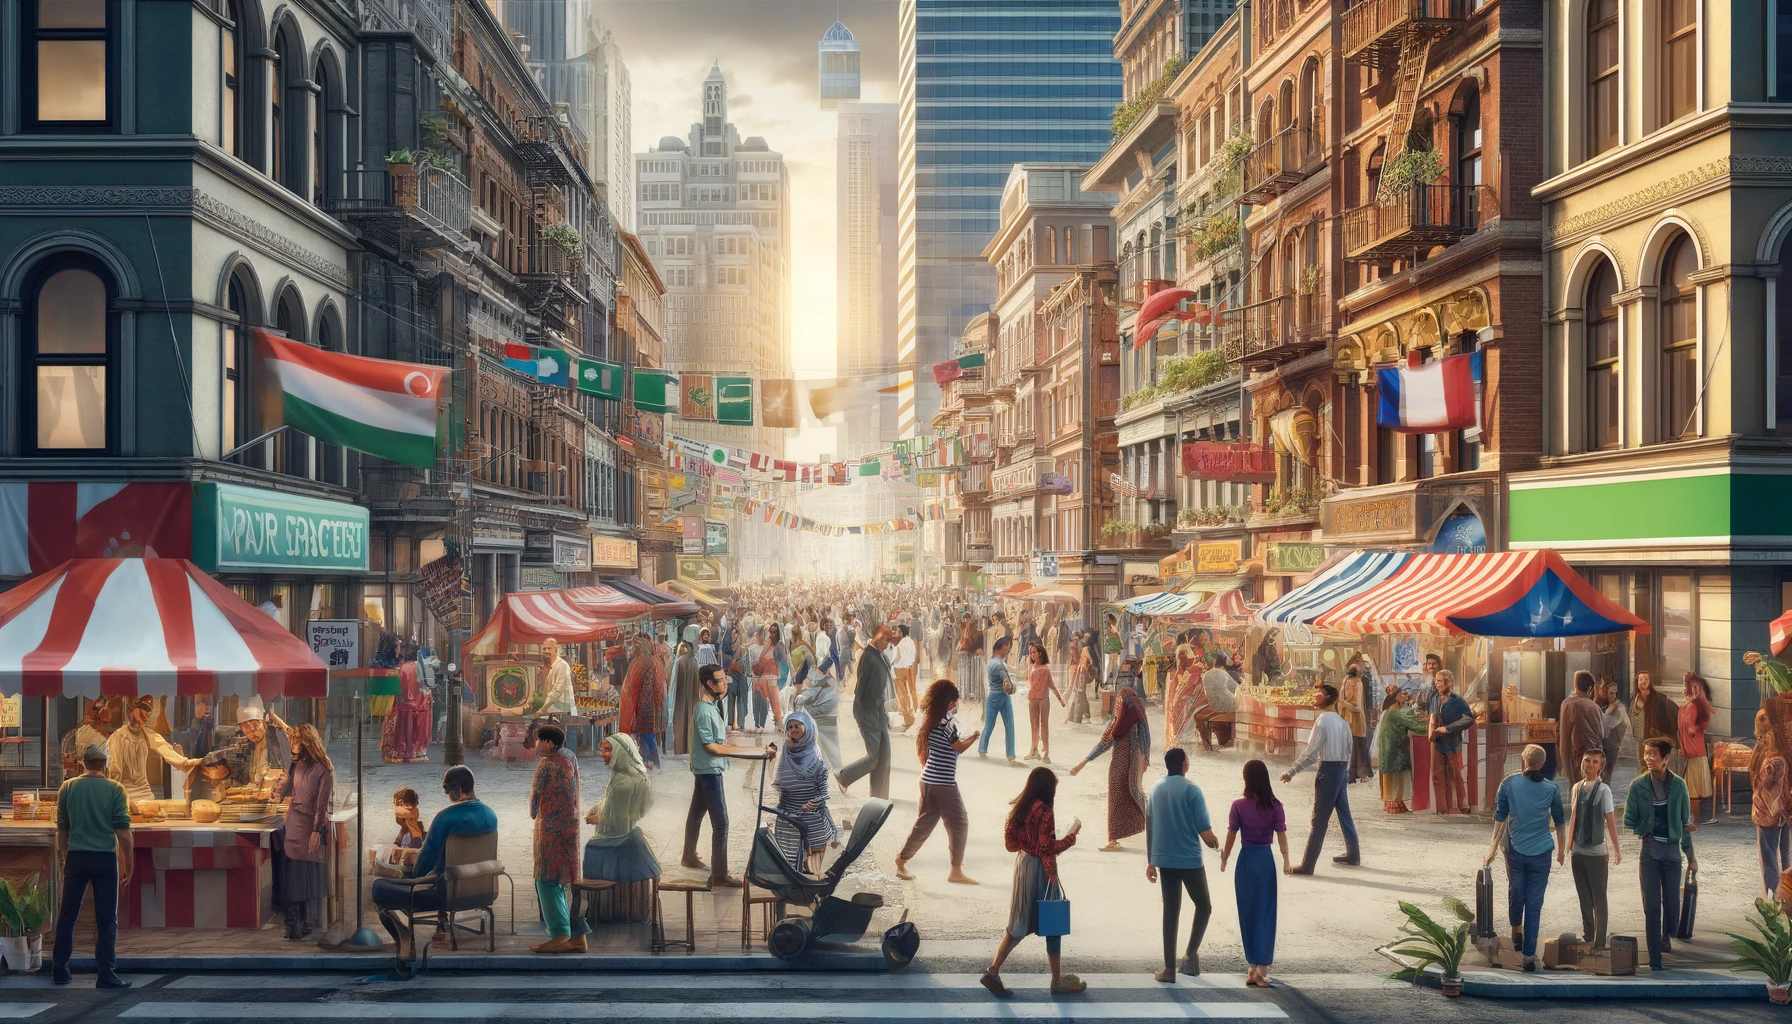
\includegraphics[width=24.89in]{images/dalle-smeltedige} \caption{Smeltedigen, tolket af en AI model}\label{fig:fig-smelte}
\end{figure}

test \citep{xie2015}.

\hypertarget{kap2}{%
\chapter{Partnerskabet og de blandede børn}\label{kap2}}

\begin{figure}
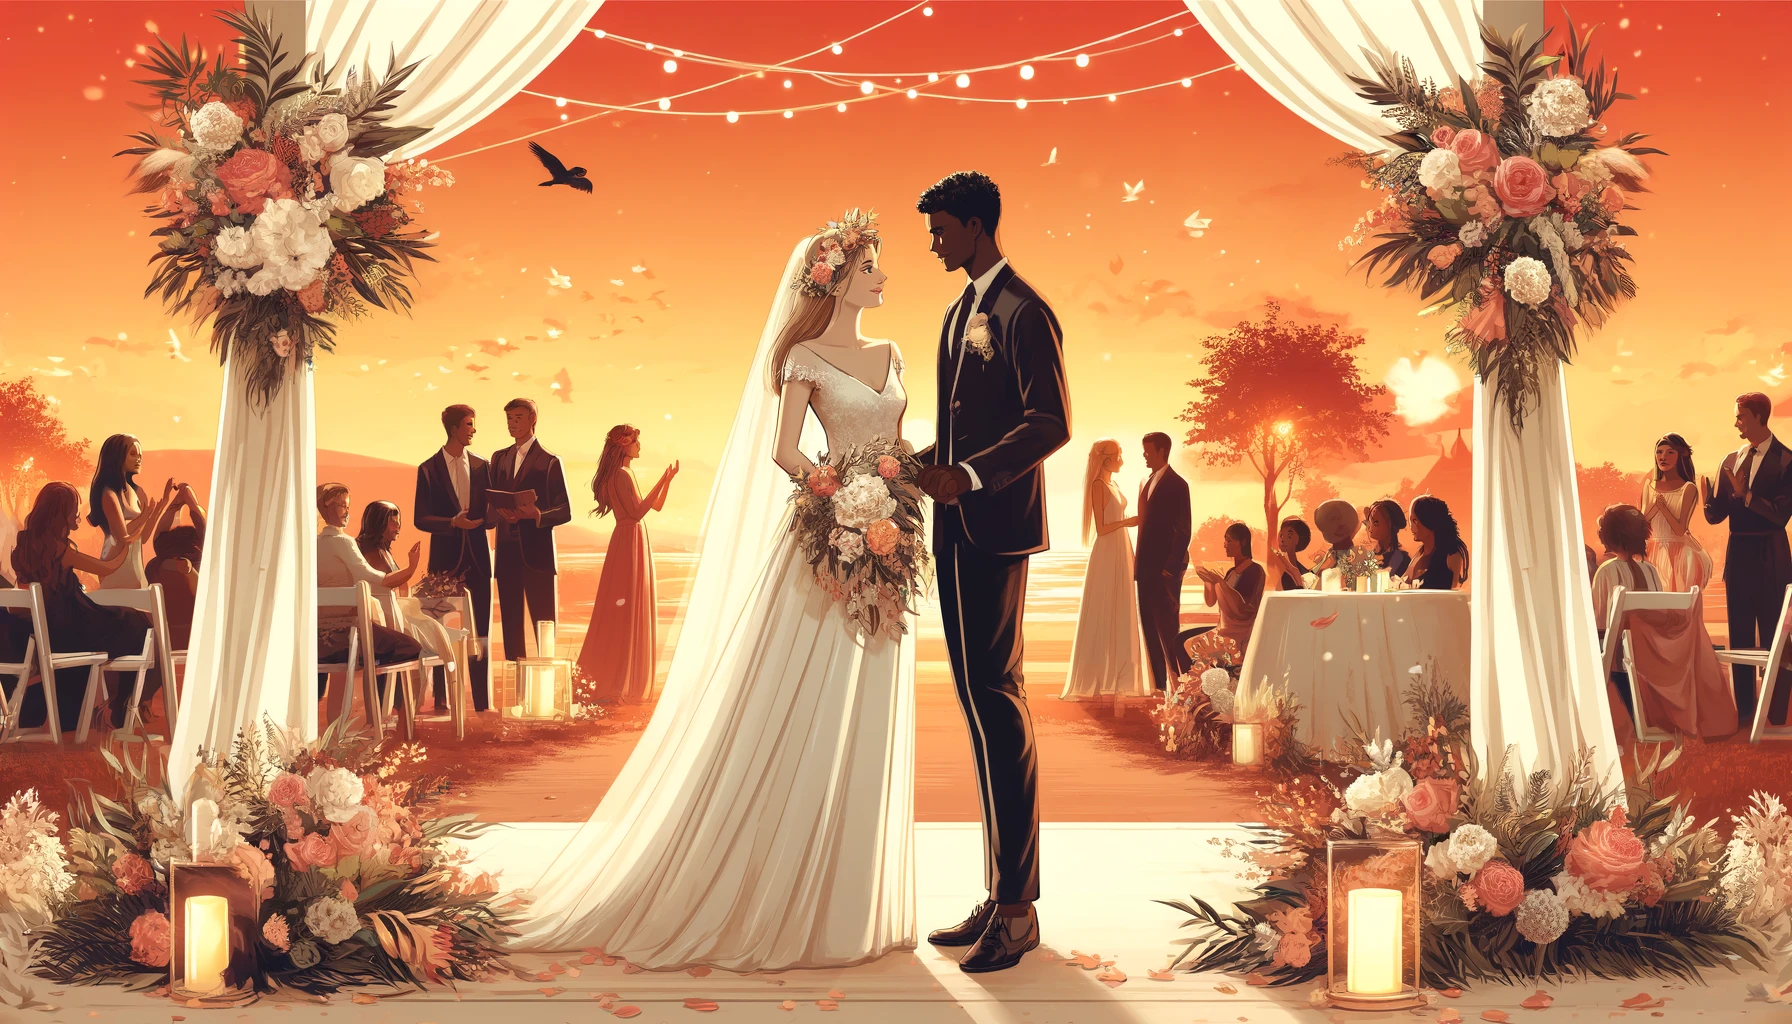
\includegraphics[width=24.89in]{images/dalle-wedding} \caption{Et blandet ægteskab, tolket af en AI model}\label{fig:fig-partner}
\end{figure}

\hypertarget{kap3}{%
\chapter{Grundskoler som mødested}\label{kap3}}

\begin{figure}
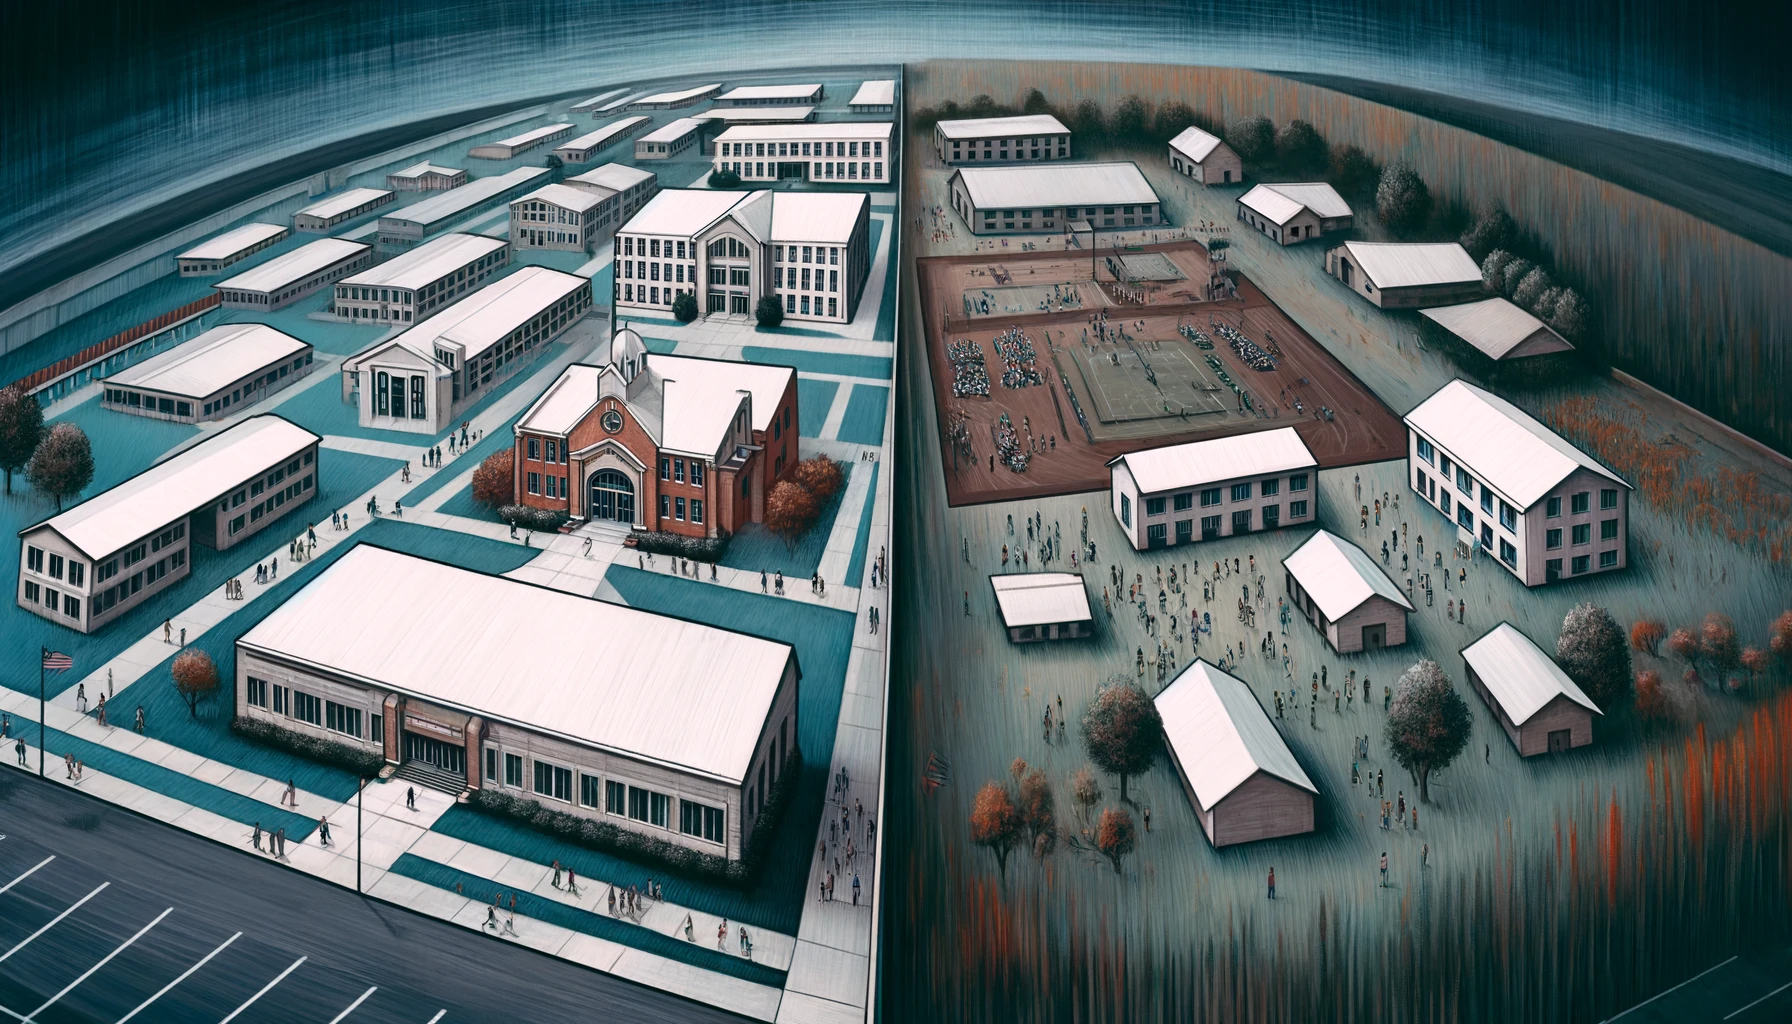
\includegraphics[width=24.89in]{images/dalle-schoolseg} \caption{Skolesegregering som det tolkes af en AI model}\label{fig:fig-schoolseg}
\end{figure}

Vi kan kryd-ref til figurer \ref{fig:fig-schoolseg}

\hypertarget{kap4}{%
\chapter{Arbejdspladser som mødested}\label{kap4}}

\begin{figure}
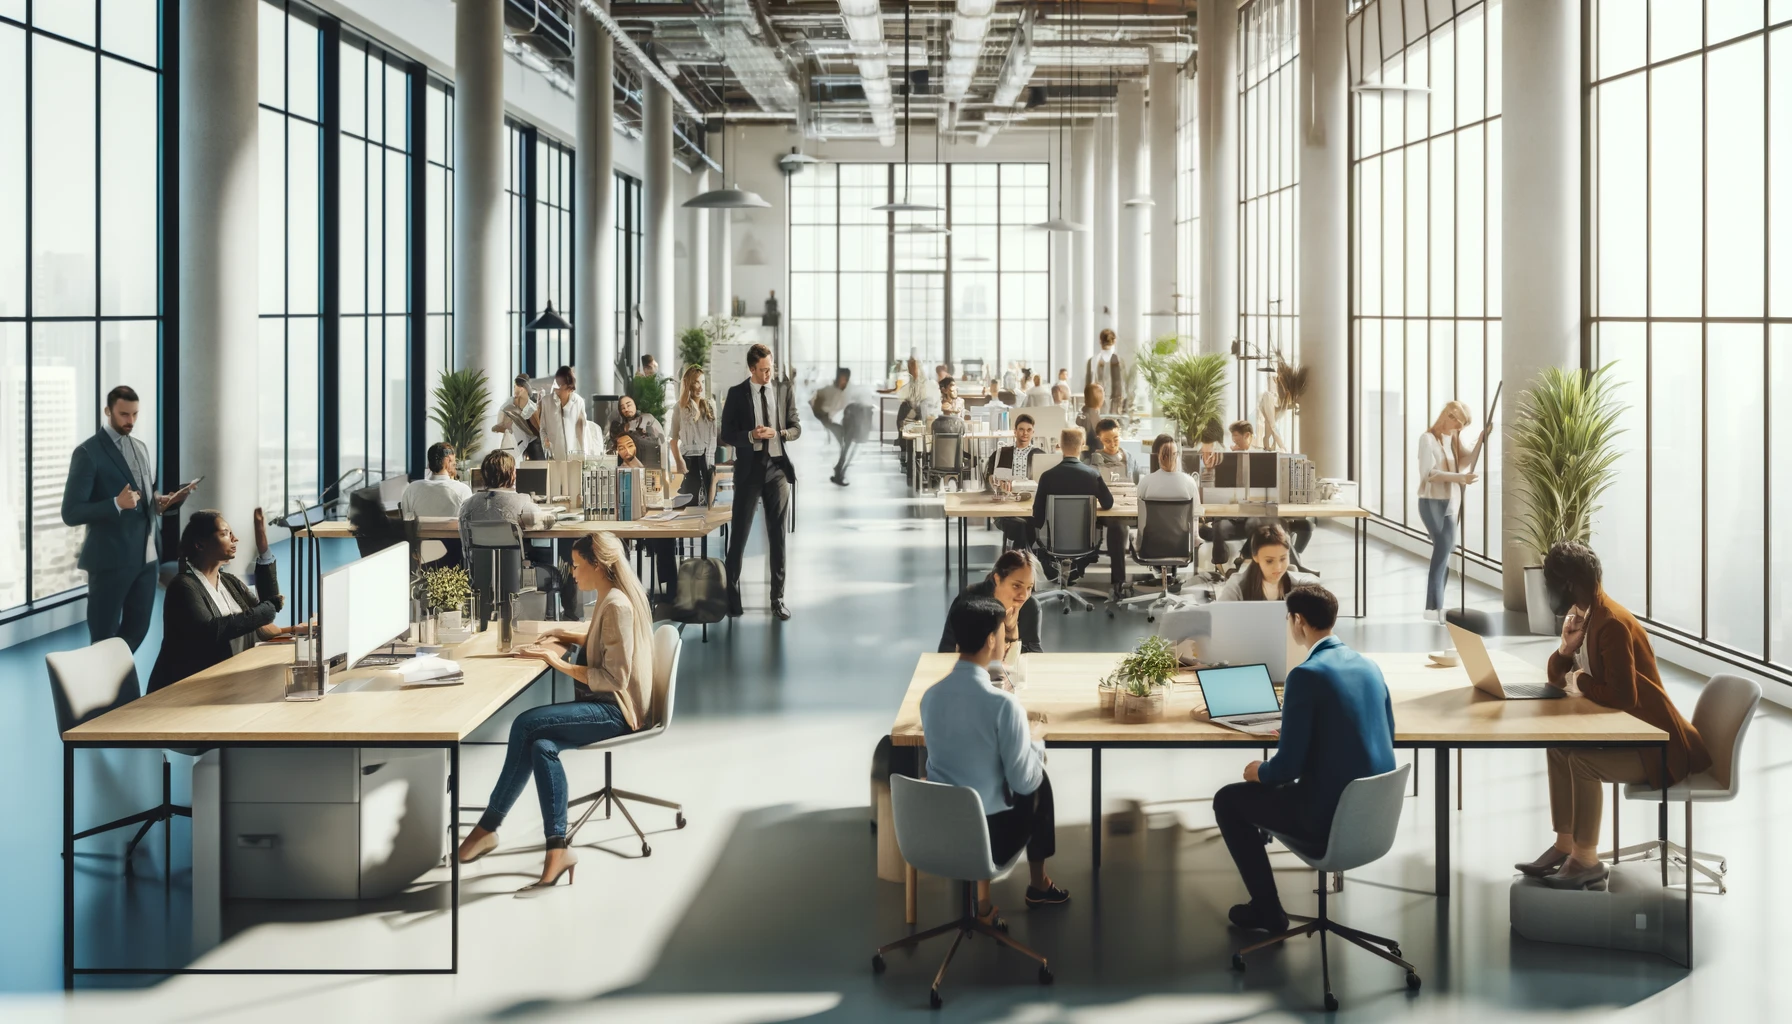
\includegraphics[width=24.89in]{images/dalle-work} \caption{En multikulturel arbejdsplads, tolket af en AI model}\label{fig:fig-work}
\end{figure}

\hypertarget{kap5}{%
\chapter{Foreninger som mødested}\label{kap5}}

\hypertarget{kap6}{%
\chapter{Venskaber -- det første skridt}\label{kap6}}

\hypertarget{kap7}{%
\chapter{Integration i et kontaktperspektiv}\label{kap7}}

test \citep{xie2015}.

\hypertarget{litteraturliste}{%
\chapter*{Litteraturliste}\label{litteraturliste}}
\addcontentsline{toc}{chapter}{Litteraturliste}

\hypertarget{appendix-bilag}{%
\appendix}


\hypertarget{bilag1}{%
\chapter{Første bilag\ldots{}}\label{bilag1}}

This will be Appendix A.

\hypertarget{bilag2}{%
\chapter{Andet bilag\ldots{}}\label{bilag2}}

This will be Appendix B.

  \bibliography{book.bib,packages.bib}

\end{document}
